\subsection{Diseño}

La etapa de diseño de este incremento se centró en la definición de las estructuras de datos, los criterios de selección y la identificación del tipo de algoritmo a emplear, así como en la especificación del comportamiento y los resultados esperados del sistema.

\textbf{En primer lugar}, se representó un instrumento mediante un vector

\[
I = [n_1, n_2, ..., n_k]
\]

donde \(k\) es el número de cuerdas del instrumento y \(n_i\) representa la nota al aire de la cuerda \(i\). De este modo, cada índice del vector corresponde a una cuerda del instrumento.

\textbf{En segundo lugar}, se representaron las combinaciones de trastes posibles mediante un vector

\[
C = [C_1, C_2, ..., C_k]
\]

donde \(k\) es el número de cuerdas del instrumento y cada elemento \(C_i\) contiene los trastes posibles para la cuerda \(i\). Cada \(C_i\) se define como un vector de trastes posibles:

\[
C_i = [f_{i1}, f_{i2}, ..., f_{im}]
\]

donde cada valor \(f_{im}\) representa un traste posible en la cuerda \(i\). Los valores de \(f_{im}\) se interpretan de la siguiente forma:

\[
f_{im} =
\begin{cases}
-1 & \text{cuerda muteada} \\
0 & \text{cuerda al aire} \\
n & \text{traste } n
\end{cases}
\]

De este modo, cada posición del vector principal corresponde a una cuerda del instrumento y contiene los trastes en los que aparecen las notas del acorde.

\textbf{En tercer lugar}, se representó el diagrama de un acorde mediante un vector

\[
D = [f_1, f_2, ..., f_k]
\]

donde \(k\) es el número de cuerdas del instrumento y \(f_i\) representa el traste pulsado en la cuerda \(i\). Cada valor del vector indica la posición del traste que debe pulsarse en la cuerda correspondiente, utilizando los mismos criterios de representación definidos anteriormente para las cuerdas muteadas, al aire o pulsadas.

\textbf{En cuarto lugar}, utilizando los vectores anteriores, se diseñó un proceso básico a través del cual obtener el diagrama de un acorde:

\begin{enumerate}
    \item Se construye el vector instrumento \(I\)\, que contiene las notas al aire de cada cuerda.
    \item Se define el acorde acorde objetivo.
    \item Se extraen del acorde la nota raíz y la cualidad.
    \item Se construye una escala cromática tomando como tónica la nota raíz del acorde.
    \item Utilizando la escala cromática y las distancias definidas por la cualidad del acorde, se seleccionan las notas que lo conforman.
    \item Se construye el vector de combinaciones \(C\)\, que para cada cuerda del instrumento contiene los trastes en los en los que aparecen las notas del acorde dentro de una profundidad de búsqueda de cuatro trastes.
    \item A partir del vector combinaciones, s egeneran las distintas combinaciones posibles de trastes, cada una representada mediante un vector \(D\)\ que corresponde a un diagrama de acorde.
\end{enumerate}

Para comprobar la efectividad del proceso anterior, se puso a prueba para la obtencion de los diagramas del acorde de \textit{GMayor} \figref{fig:builddiagram_it2_gmayor}.

\begin{figure}[H]
    \centering
    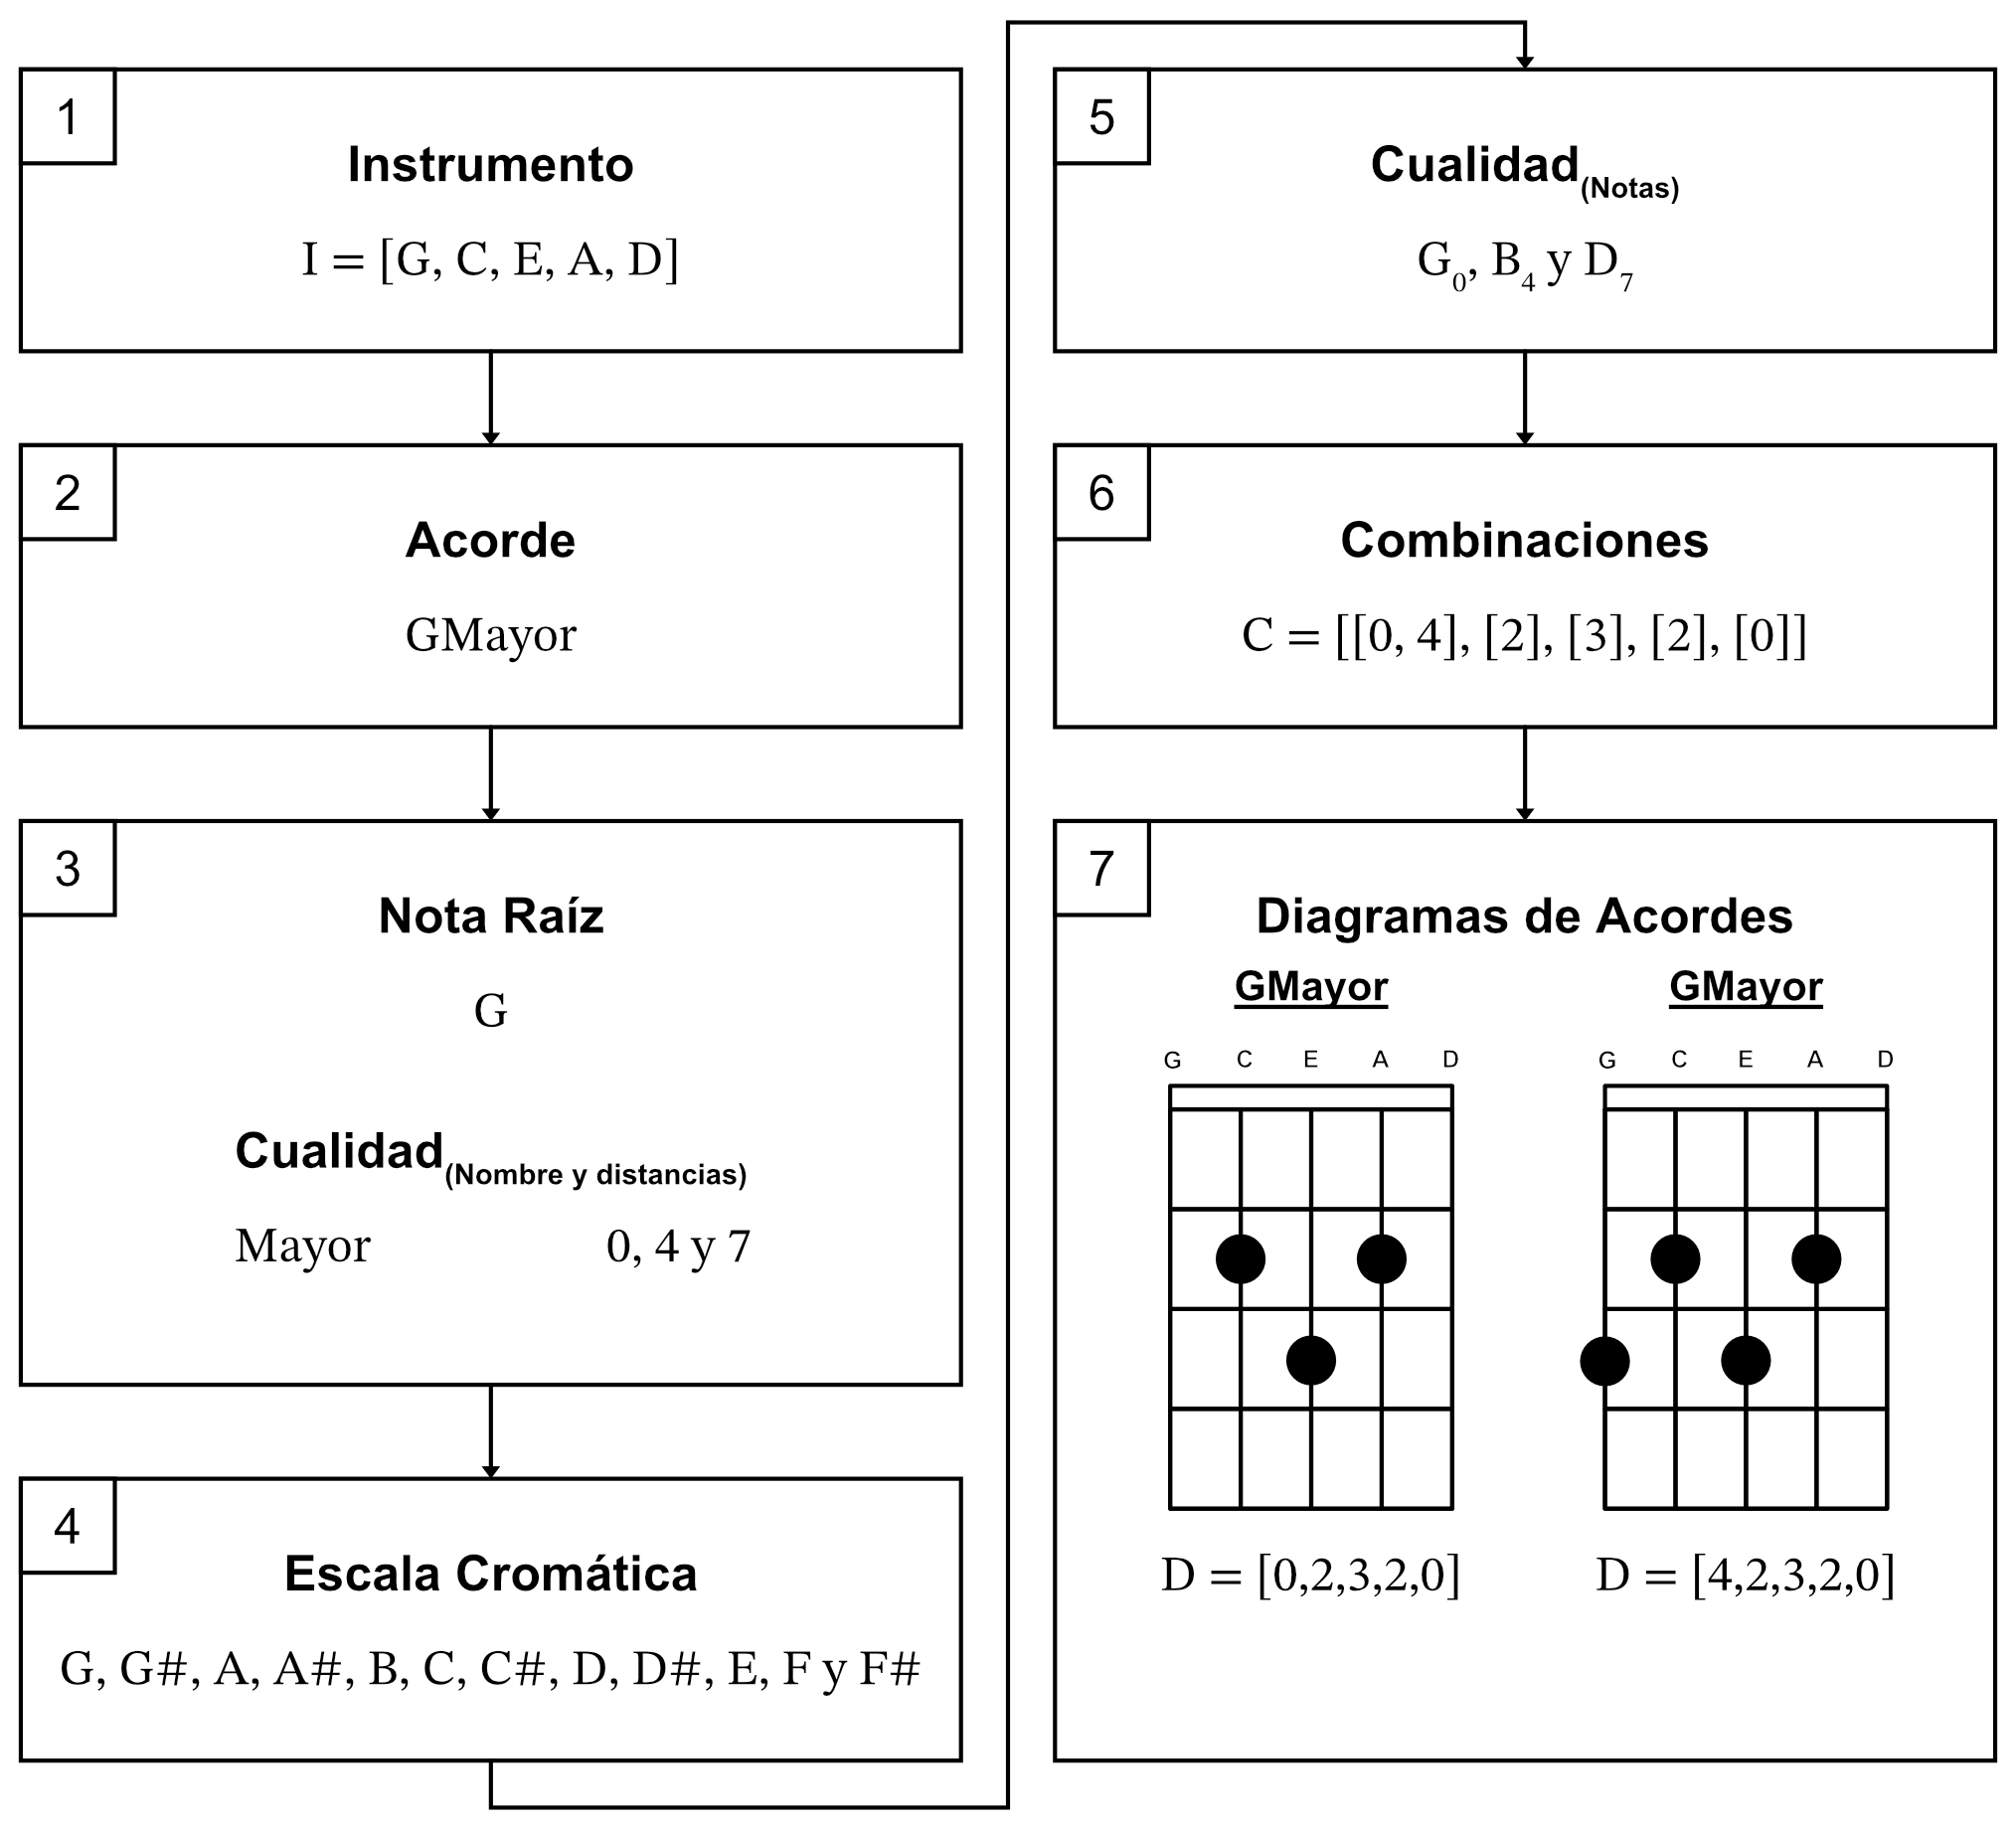
\includegraphics[width=0.8\textwidth]{Ilustraciones/desarrollo/incremento2/diseño/builddiagram_it2_gmayor.jpg}
    \caption{Construcción de diagramas del acorde de \textit{GMayor} con vectores}\label{fig:builddiagram_it2_gmayor}
\end{figure}

\textbf{En quinto lugar}, el proceso anterior no garantiza que las combinaciones sean correctas musicalmente \textit{(i.e. pueden generarse combinaciones con notas repetidas o ausentes)} ni físicamente practicables \textit{(i.e. puede haber más trastes que dedos disponibles)}. Por ello, se definió un conjunto de criterios de selección para evaluar y priorizar las combinaciones generadas:

\begin{enumerate}
    \item \textbf{Practicabilidad física:}
    \begin{itemize}
        \item El acorde debe poder tocarse utilizando como máximo cuatro dedos.
        \item Cada cuerda pulsada o muteada suma un dedo.
        \item Las cuerdas al aire no suman dedos.
        \item La cejilla suma un dedo para todas las cuerdas que tengan el mismo traste pulsado.
    \end{itemize}
    
    \item \textbf{Facilidad de reproducción:} donde se priorizan diagramas con:
    \begin{itemize}
        \item Mayor número de cuerdas al aire.
        \item Menor número de dedos utilizados.
        \item Ausencia de cuerdas muteadas.
        \item Ausencia de cejilla
        \item Menor número de trastes pisados bajo cejilla.
    \end{itemize}

    \item \textbf{Correctitud musical:}
    \begin{itemize}
        \item Cada nota definida por la cualidad del acorde tiene un peso asociado.
        \item No se admiten combinaciones sin la nota raíz ni combinaciones con todas las notas iguales.
        \item Se priorizan las combinaciones que incluyen la mayor suma de pesos de las notas.
    \end{itemize}
\end{enumerate}

Con estos criterios, se diseñó un sistema de puntuación por \textbf{penalizaciones}, donde se suma la dificultad de reproducción y las carencias en correctitud musical. La selección de la \textbf{mejor combinación} se realiza eligiendo aquella con la \textbf{mínima puntuación}.

\begin{itemize}
    \item La \textbf{ramificación} realiza la \textbf{búsqueda en profundidad} sobre el vector de combinaciones \(C\), generando variantes parciales.
    \item La \textbf{poda} controla la exploración siguiendo los criterios de selección:
            \begin{enumerate}
                \item \textbf{Poda temprana}: se descartan ramas que no cumplen la practicabilidad física.
                \item \textbf{Poda intermedia}: se descartan ramas cuya puntuación en facilidad de reproducción es peor que la mejor variante conocida hasta el momento.
            \end{enumerate}
    \item La \textbf{actualización de la mejor solución}: cuando una variante completa tiene una puntuación total (facilidad de reproducción + correctitud musical) mejor que la mejor encontrada hasta el momento, se actualiza la solución óptima.
\end{itemize}

La lógica anterior fue puesta a prueba mediante la representación de un árbol de búsqueda, aplicando las operaciones mencionadas para la obtención de diagramas de los acordes de \textit{CMayor} \figref{fig:arbol_it2_cmayor} y \textit{BMayor} \figref{fig:arbol_it2_bmayor}, con el objetivo de analizar el comportamiento del árbol y la efectividad del proceso de poda.

\begin{figure}[H]
    \centering
    \begin{subfigure}{\textwidth}
        \centering
        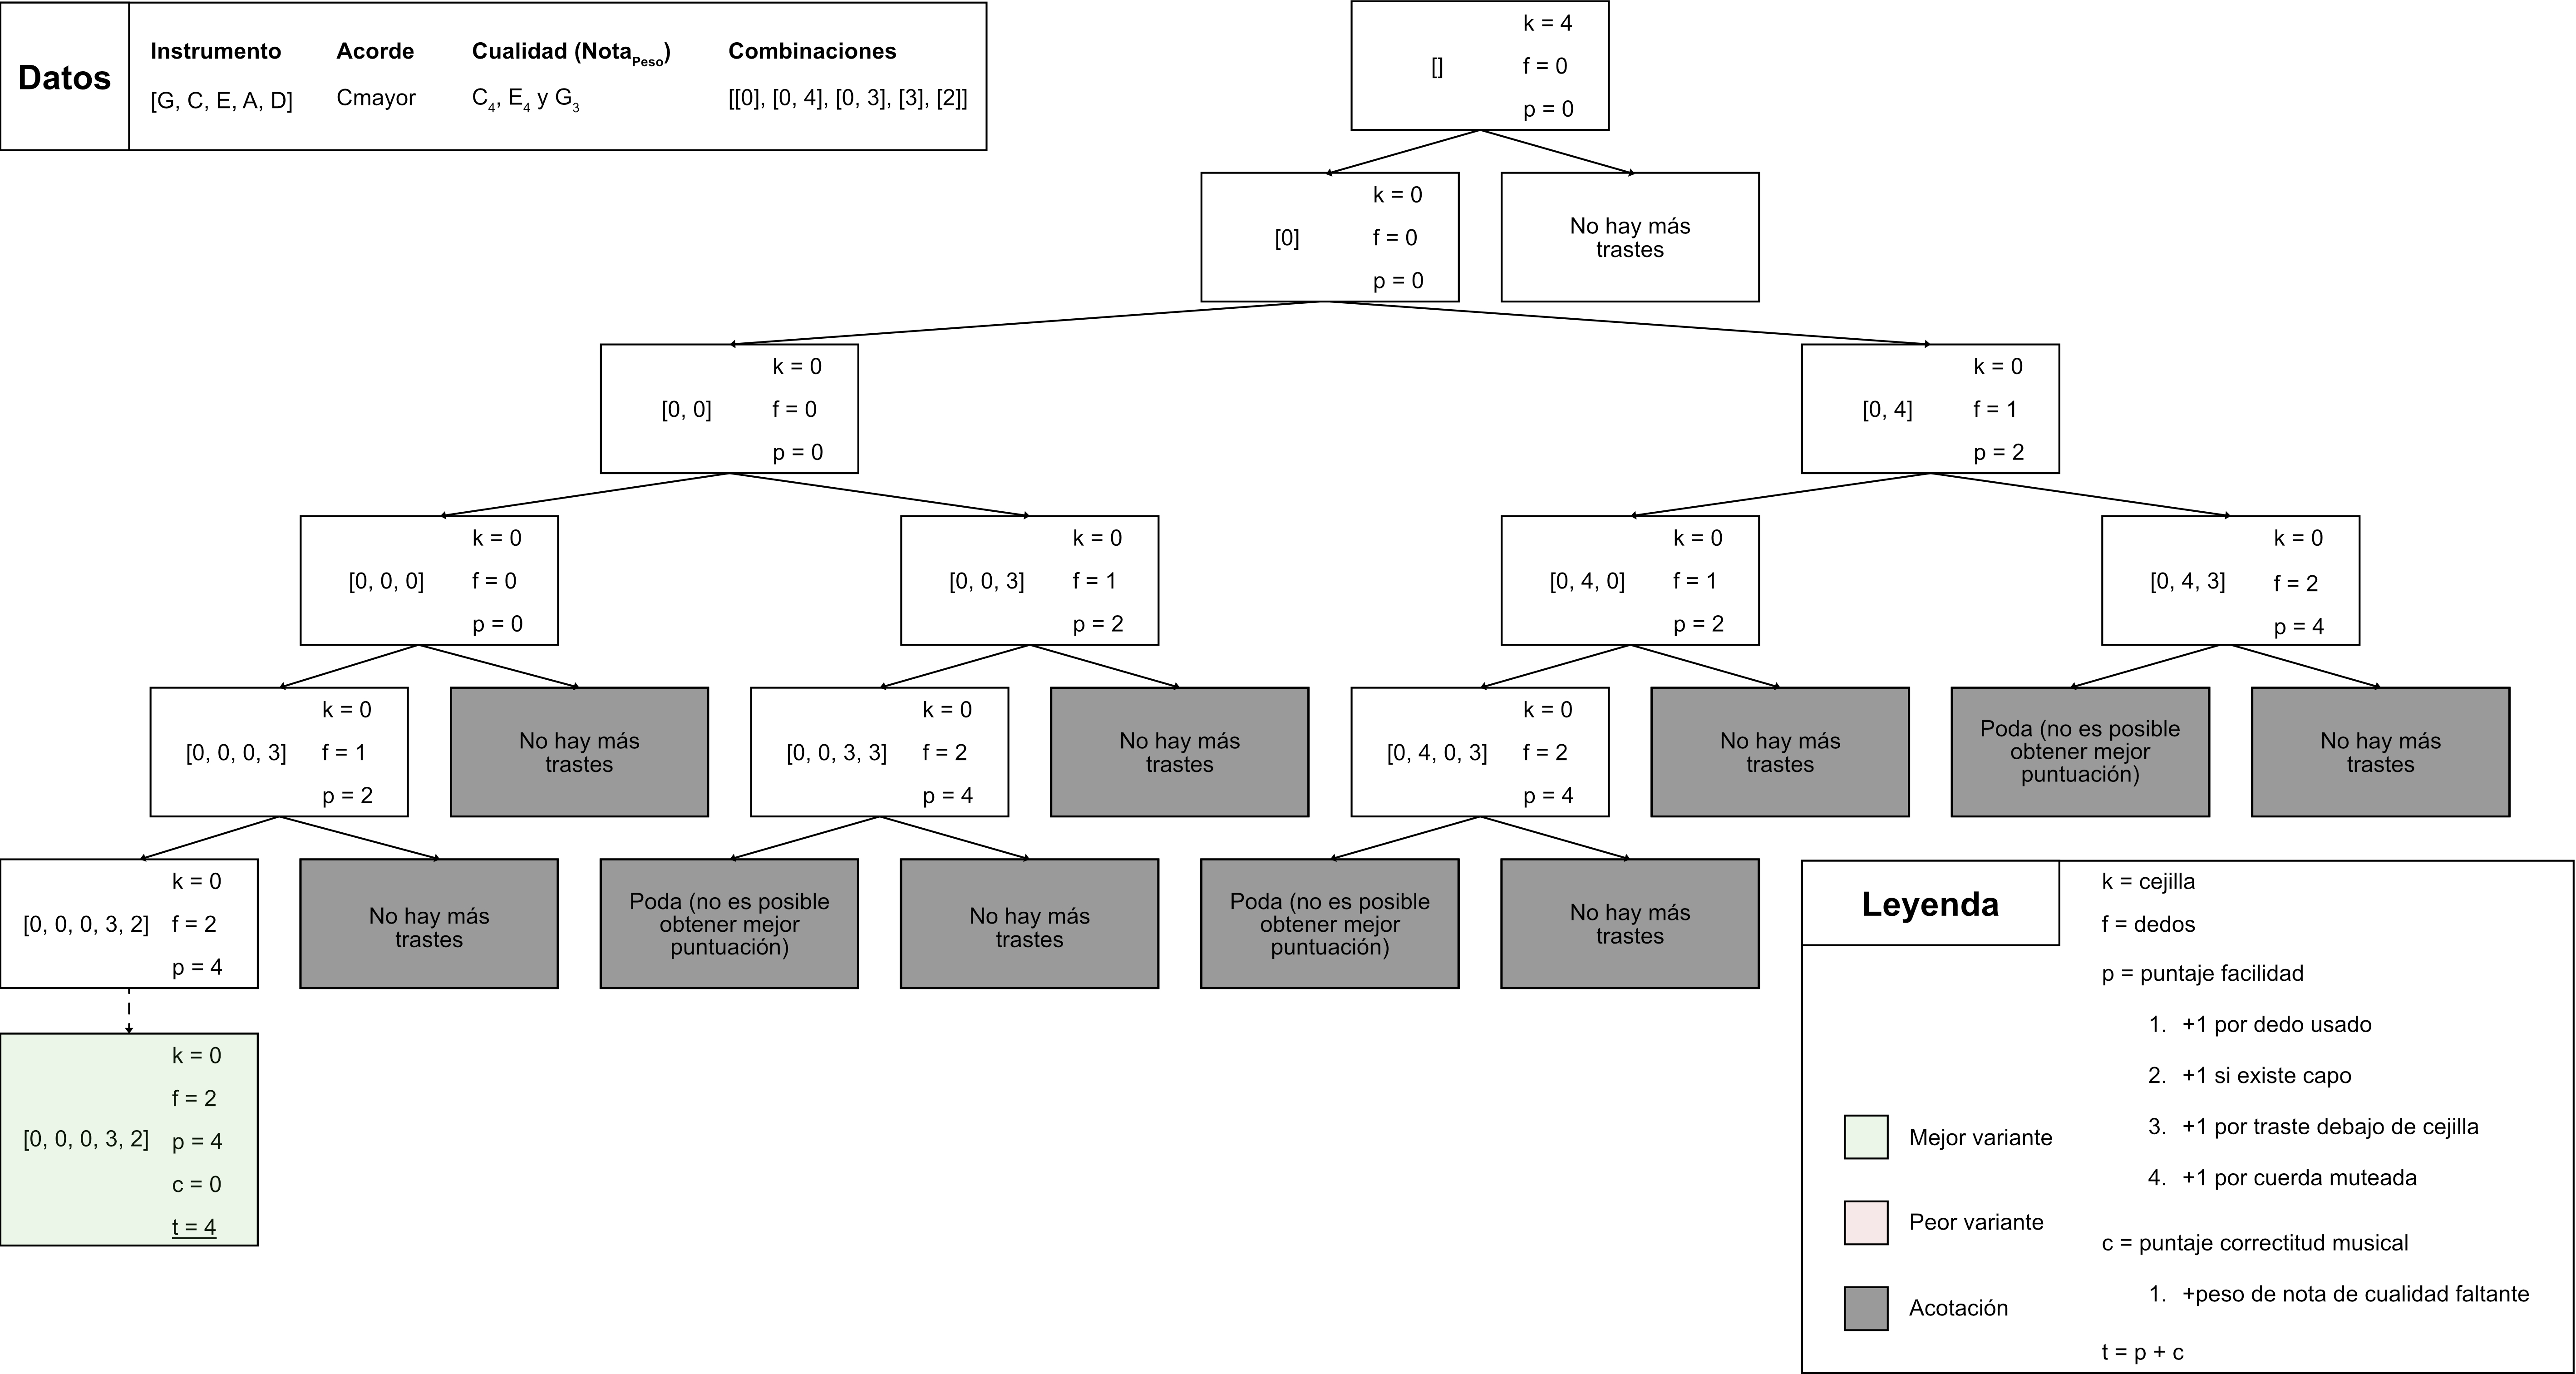
\includegraphics[width=\textwidth]{Ilustraciones/desarrollo/incremento2/diseño/arbol_it2_cmayor.jpg}
        \caption{Árbol de búsqueda resultante para el diagrama del acorde de \textit{CMayor}}
        \label{fig:arbol_it2_cmayor}
    \end{subfigure}

    \begin{subfigure}{\textwidth}
        \centering
        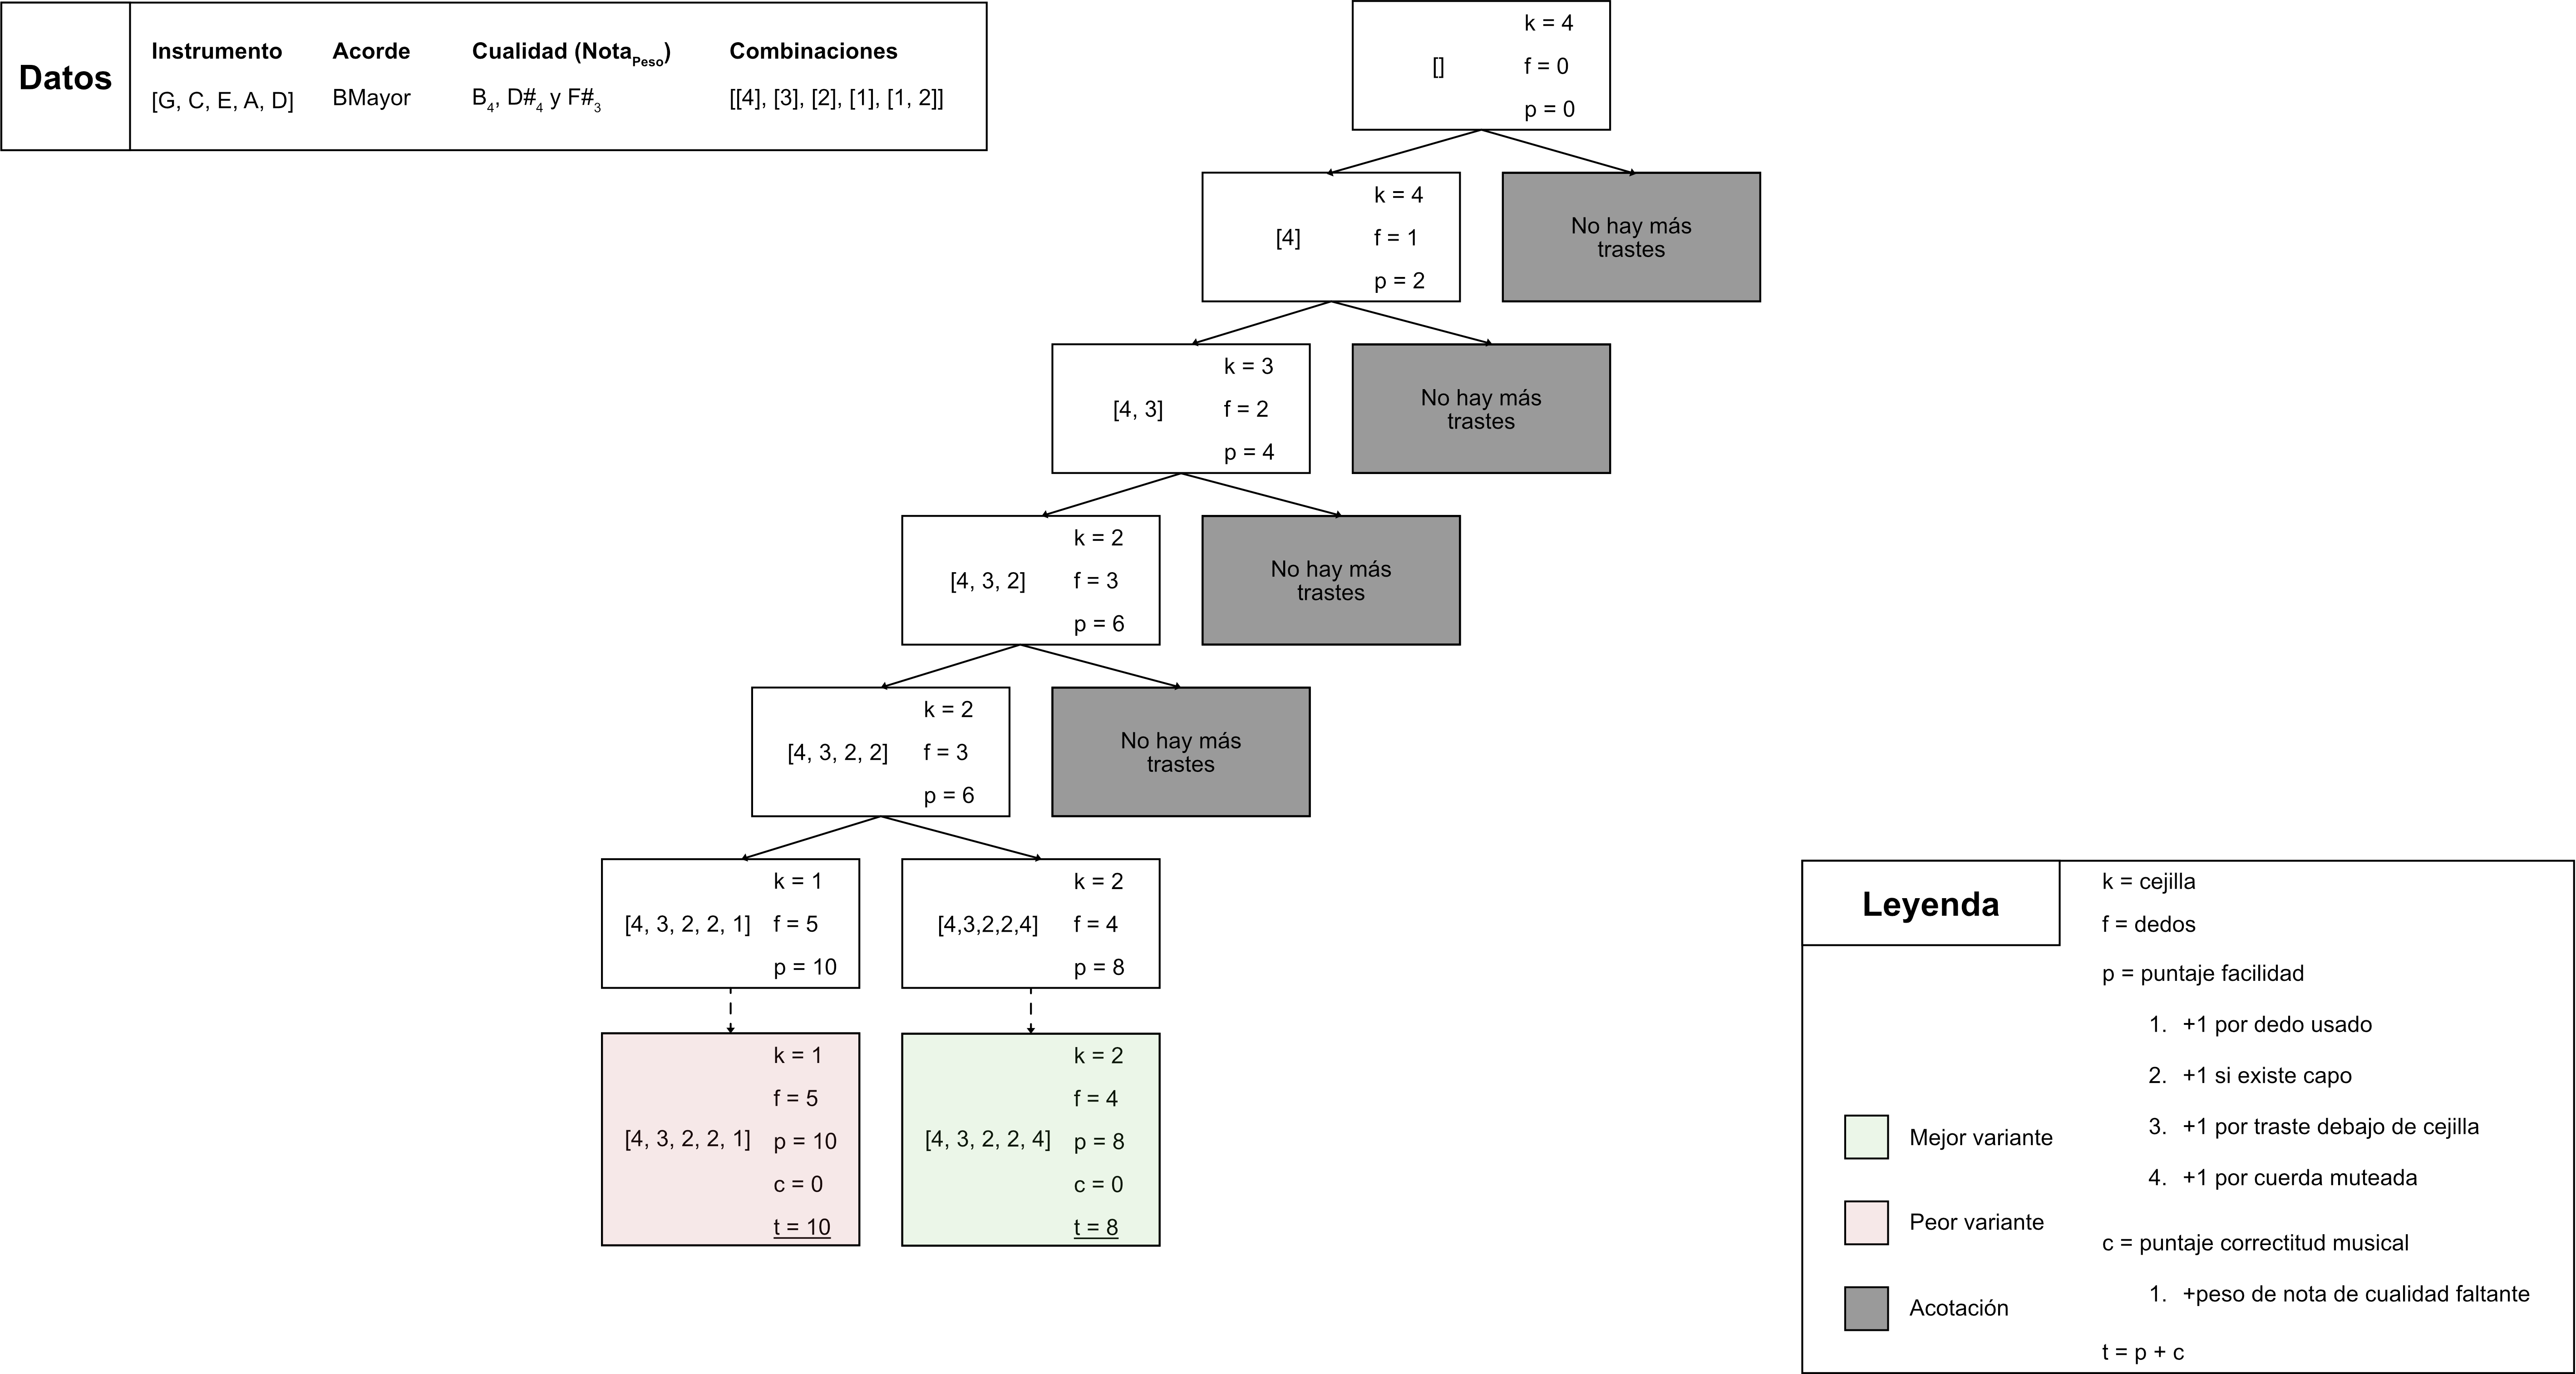
\includegraphics[width=\textwidth]{Ilustraciones/desarrollo/incremento2/diseño/arbol_it2_bmayor.jpg}
        \caption{Árbol búsqueda resultante para el diagrama del acorde de \textit{BMayor}}
        \label{fig:arbol_it2_bmayor}
    \end{subfigure}
    \caption{Árbol de búsqueda resultante del algoritmo de calculo de diagramas de acordes}\label{fig:arbol_it2}
\end{figure}